\section{Wormholes and tachyon condensation}\label{sec:wormholes}

The wormhole solutions connect two asymptotic AdS regions of the same radius, which suggests that there are two quantum field theories with the same number of degrees of freedom that are decoupled from each other in the $N\to \infty$ limit, where the gravitational dual becomes free. The main difference that one observes between the two regions connected through the wormhole is that the orientation of the boundary is reversed, which is also reflected in the superpotential having an opposite sign in each asymptotic region. When the AdS solutions at the critical points of the superpotential have a dual interpretation in terms of a brane intersection, this suggests that each boundary would correspond to an opposite orientation of the branes and thus one boundary would correspond to a stack of branes and the other to a stack of anti-branes. 
 
The observations made above hint at the possibility that the wormhole solution is dual to a state where tachyon condensation connects branes with anti-branes. An analogous non-gravitational example is the description of chiral symmetry breaking in the Sakai-Sugimoto model when D8 branes and anti-branes reconnect in the gravity dual \cite{Sakai:2004cn,Casero:2007ae,Dhar:2007bz}. With this interpretation, the geometry of the wormhole could be as described in Figure \ref{fig:tachyon}, similar to the one discussed in \cite{Balasubramanian:2020ffd} for two stacks of D3 branes. One starts with an asymptotically flat geometry and two separated throats corresponding to each of the stacks. Then the throats become connected at the interior by cutting and gluing them, and the asymptotically flat region is removed by taking the near-horizon limit. Nevertheless, the solutions discussed here present two differences with respect to the construction of \cite{Balasubramanian:2020ffd}: first, the adhesion of the throats does not require an inversion; second, the near-horizon limit here would be such that only the low-energy degrees of freedom living in the wormhole remain, and the two throats do not join in a larger throat with a single AdS boundary. Note that, before taking the near-horizon limit, there would be an attractive force between the two throats that renders the system unstable. However, the near-horizon limit removes the degrees of freedom corresponding to the center of mass motion of each of the throats and this instability would disappear.

\begin{figure}[ht!]
	\centering
	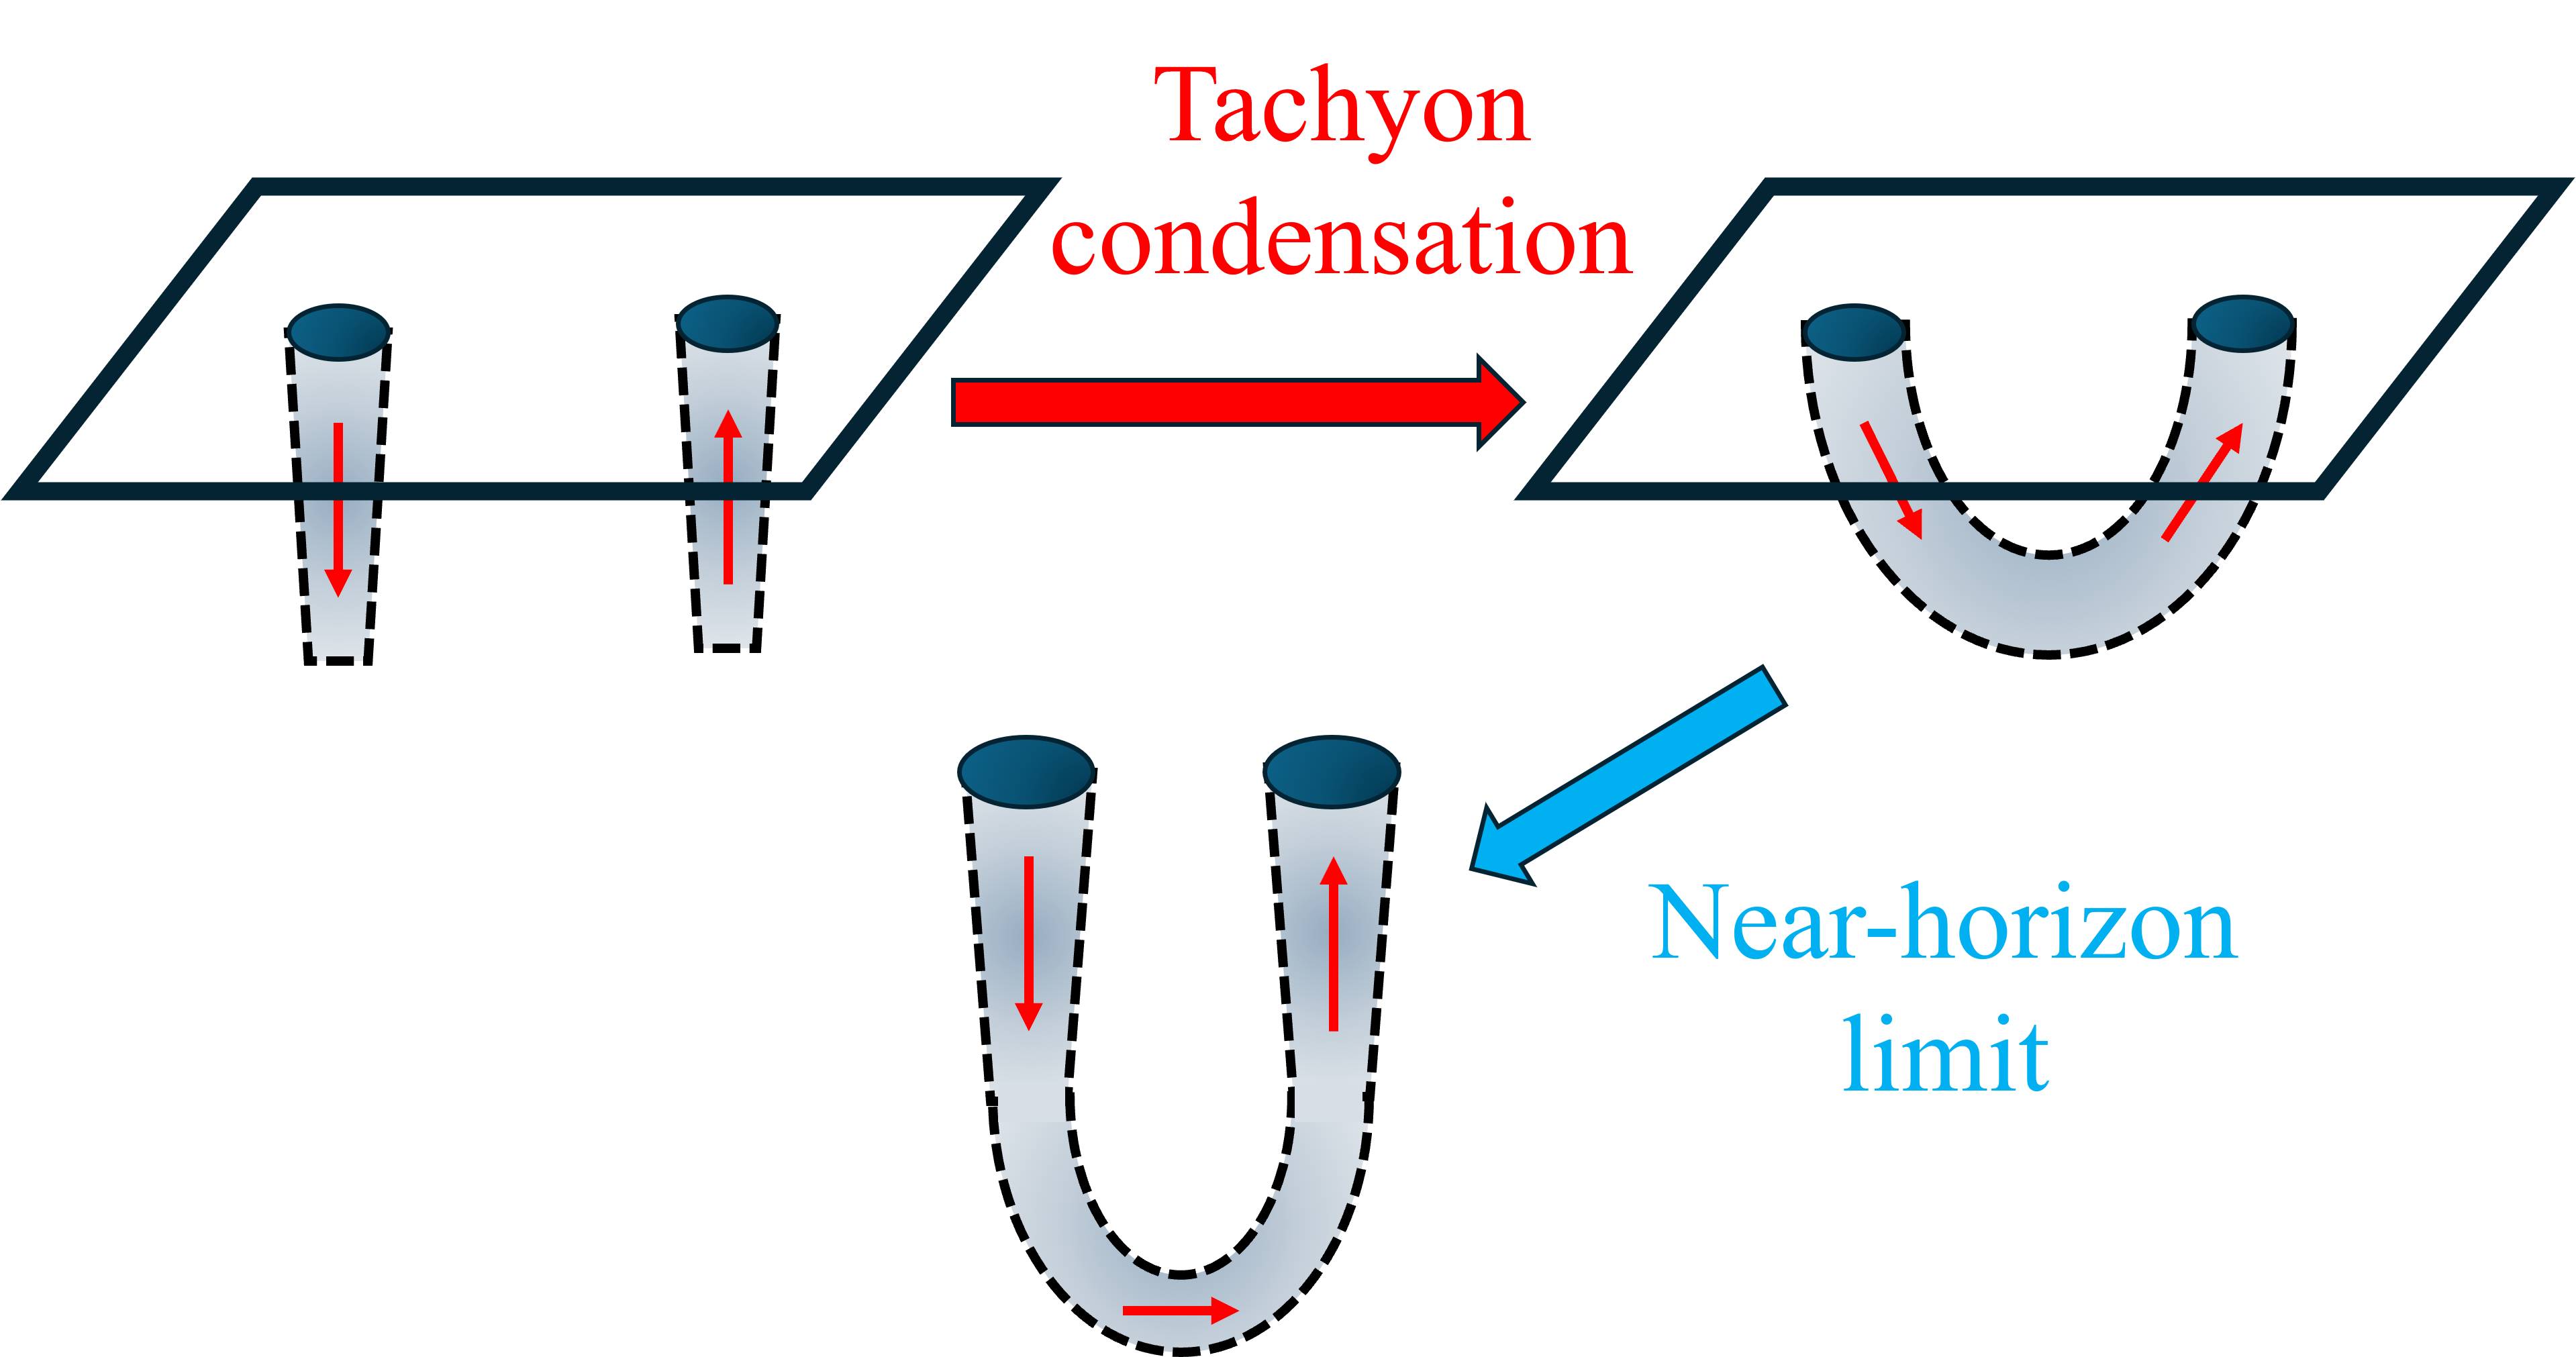
\includegraphics[width=0.7\linewidth]{tachyoncondensation.png} % paper/images/: hand-made, not generated
	\caption{Possible formation of the wormhole. Two stacks of branes and anti-branes form throats inside an asymptotically flat spacetime when they backreact. Condensation of the open string tachyon makes the two throats connect forming a wormhole. In the near-horizon limit the geometry is restricted to the interior of the wormhole, that connects two asymptotically AdS spacetimes.}
	\label{fig:tachyon}
\end{figure}

Let us provide a concrete example that exhibits some of the characteristics mentioned above. We do not claim that this example is the actual holographic dual of the flows we found, but it might serve to illustrate the connection between the analytic extension of the fields and tachyon condensation.

An effective action for a system of D-branes and anti D-branes was proposed in \cite{Sen:2003tm,Garousi:2004rd} (see also \cite{Kraus:2000nj,Takayanagi:2000rz,Jones:2002sia,Jatkar:2000ei,Hikida:2000cp}). It takes the form of a generalization of the Dirac-Born-Infeld and Wess-Zumino actions including the open string tachyon. For D$p$-branes, the low-energy expansion results in two copies of the maximally supersymmetric theory in $p+1$ dimensions plus a complex tachyon field, with an action 
\begin{equation}
	S_{D\bar{D}}=S_{\text{SYM}}^{(1)}+S_{\text{SYM}}^{(2)}+S_{\rm tach}\ ,
\end{equation}
where, assuming an Abelian configuration of $N$ $D\bar{D}$ pairs,
\begin{equation}
	S_{\rm tach}=-N(2\pi \alpha')^2T_{Dp}\int \dd^{p+1}x \left(\partial_\mu\overline{T}\partial^\mu T+\frac{1}{4}\partial_\mu X\partial^\mu X+V\right),
\end{equation}
where $T$ is the tachyon and $X=X^{(1)}-X^{(2)}$ is the separation between the stacks of branes and anti-branes. The potential is%
\footnote{Before expanding in $\alpha'$, the potential decays exponentially at large values of the tachyon to the true minimum at $T\to \infty$. This behaviour is lost in the low-energy expansion.}
\begin{equation}
	V(|T|,X)=|T|^2\left( X^2-\frac{1}{2\alpha'}\right)+v_4 (|T|^2)^2+V_0\ .
\end{equation}
The first two terms correspond to the mass of the lowest energy excitation of a string extended between the brane and the anti-brane. The quartic term depends on details of the tachyon potential which are not fully known, but, from the proposals that have been put forward, one expects to have $v_4>0$ and of order one. A physical separation between the two stacks of the order of the size of the throats, $L$, corresponds to $X^2\sim L^2/(\alpha')^2\gg 1/\alpha'$ when the number of branes is large enough. For instance, in the case of D3 branes, $L$ gives the AdS radius of the near-horizon geometry, and it is related through the holographic dictionary to the 't Hooft coupling of the field theory $X^2\sim \sqrt{\lambda}/\alpha'\gg 1/\alpha'$. In this case, the tachyon is stabilized at $T=0$ and there is no condensation, the brane and anti-branes are completely decoupled at low energies. However, if we now allow the analytic extension to purely imaginary values of the separation, $X\to X=i Y$, the $T=0$ point becomes a maximum and tachyon condensation is triggered. The wormhole would be the endpoint of the condensation in the holographic dual description.

